\documentclass[man]{apa6}
\usepackage{lmodern}
\usepackage{amssymb,amsmath}
\usepackage{ifxetex,ifluatex}
\usepackage{fixltx2e} % provides \textsubscript
\ifnum 0\ifxetex 1\fi\ifluatex 1\fi=0 % if pdftex
  \usepackage[T1]{fontenc}
  \usepackage[utf8]{inputenc}
\else % if luatex or xelatex
  \ifxetex
    \usepackage{mathspec}
  \else
    \usepackage{fontspec}
  \fi
  \defaultfontfeatures{Ligatures=TeX,Scale=MatchLowercase}
\fi
% use upquote if available, for straight quotes in verbatim environments
\IfFileExists{upquote.sty}{\usepackage{upquote}}{}
% use microtype if available
\IfFileExists{microtype.sty}{%
\usepackage{microtype}
\UseMicrotypeSet[protrusion]{basicmath} % disable protrusion for tt fonts
}{}
\usepackage{hyperref}
\hypersetup{unicode=true,
            pdftitle={Domain-specific working memory loads selectively increase negative interpertations of surprised facial expressions},
            pdfauthor={Nicholas R. Harp~\& Maital Neta},
            pdfkeywords={ambiguity, working memory, bias},
            pdfborder={0 0 0},
            breaklinks=true}
\urlstyle{same}  % don't use monospace font for urls
\usepackage{graphicx,grffile}
\makeatletter
\def\maxwidth{\ifdim\Gin@nat@width>\linewidth\linewidth\else\Gin@nat@width\fi}
\def\maxheight{\ifdim\Gin@nat@height>\textheight\textheight\else\Gin@nat@height\fi}
\makeatother
% Scale images if necessary, so that they will not overflow the page
% margins by default, and it is still possible to overwrite the defaults
% using explicit options in \includegraphics[width, height, ...]{}
\setkeys{Gin}{width=\maxwidth,height=\maxheight,keepaspectratio}
\IfFileExists{parskip.sty}{%
\usepackage{parskip}
}{% else
\setlength{\parindent}{0pt}
\setlength{\parskip}{6pt plus 2pt minus 1pt}
}
\setlength{\emergencystretch}{3em}  % prevent overfull lines
\providecommand{\tightlist}{%
  \setlength{\itemsep}{0pt}\setlength{\parskip}{0pt}}
\setcounter{secnumdepth}{0}
% Redefines (sub)paragraphs to behave more like sections
\ifx\paragraph\undefined\else
\let\oldparagraph\paragraph
\renewcommand{\paragraph}[1]{\oldparagraph{#1}\mbox{}}
\fi
\ifx\subparagraph\undefined\else
\let\oldsubparagraph\subparagraph
\renewcommand{\subparagraph}[1]{\oldsubparagraph{#1}\mbox{}}
\fi

%%% Use protect on footnotes to avoid problems with footnotes in titles
\let\rmarkdownfootnote\footnote%
\def\footnote{\protect\rmarkdownfootnote}


  \title{Domain-specific working memory loads selectively increase negative interpertations of surprised facial expressions}
    \author{Nicholas R. Harp\textsuperscript{1}~\& Maital Neta\textsuperscript{1}}
    \date{}
  
\shorttitle{DOMAIN-SPECIFIC WORKING MEMORY AND SURPRISED EXPRESSIONS}
\affiliation{
\vspace{0.5cm}
\textsuperscript{1} University of Nebraska-Lincoln}
\keywords{ambiguity, working memory, bias\newline\indent Word count: X}
\usepackage{csquotes}
\usepackage{upgreek}
\captionsetup{font=singlespacing,justification=justified}

\usepackage{longtable}
\usepackage{lscape}
\usepackage{multirow}
\usepackage{tabularx}
\usepackage[flushleft]{threeparttable}
\usepackage{threeparttablex}

\newenvironment{lltable}{\begin{landscape}\begin{center}\begin{ThreePartTable}}{\end{ThreePartTable}\end{center}\end{landscape}}

\makeatletter
\newcommand\LastLTentrywidth{1em}
\newlength\longtablewidth
\setlength{\longtablewidth}{1in}
\newcommand{\getlongtablewidth}{\begingroup \ifcsname LT@\roman{LT@tables}\endcsname \global\longtablewidth=0pt \renewcommand{\LT@entry}[2]{\global\advance\longtablewidth by ##2\relax\gdef\LastLTentrywidth{##2}}\@nameuse{LT@\roman{LT@tables}} \fi \endgroup}


\DeclareDelayedFloatFlavor{ThreePartTable}{table}
\DeclareDelayedFloatFlavor{lltable}{table}
\DeclareDelayedFloatFlavor*{longtable}{table}
\makeatletter
\renewcommand{\efloat@iwrite}[1]{\immediate\expandafter\protected@write\csname efloat@post#1\endcsname{}}
\makeatother
\usepackage{lineno}

\linenumbers

\authornote{Nicholas R. Harp, Department of Psychology, Center for Brain, Biology, and Behavior, University of Nebraska-Lincoln
Maital Neta, Department of Psychology, Center for Brain, Biology, and Behavior, University of Nebraska-Lincoln

Correspondence concerning this article should be addressed to Nicholas R. Harp, Postal address. E-mail: \href{mailto:nharp@huskers.unl.edu}{\nolinkurl{nharp@huskers.unl.edu}}}

\abstract{
Individual differences in interpretations of emotional ambiguity are a useful tool for measuring affective biases.

While trait-like, these biases are also susceptible to experimental manipulations. In the present study, we capitalize on this malleability to expand on previous research suggesting that
subjective interpretations are stable independently of cognitive load.

We tested the effects of working memory loads containing either neutral or emotional content on concurrent interpretations of surprised facial expressions.

Here we show that interpretations of surprise are more negative during maintenance of working memory loads with emotional content compared to those with neutral content.

Two or three sentences explaining what the \textbf{main result} reveals in direct comparison to what was thought to be the case previously, or how the main result adds to previous knowledge.

One or two sentences to put the results into a more \textbf{general context}.

Two or three sentences to provide a \textbf{broader perspective}, readily comprehensible to a scientist in any discipline.


}

\begin{document}
\maketitle

\hypertarget{introduction}{%
\section{Introduction}\label{introduction}}

Facial expressions are rich with affective information, and correctly interpreting these social cues is critical for successfully navigating the social world. In fact, facial expressions are seen across cultures ({\textbf{???}}) and some evidence suggests expressions are innate (cite). Often, facial expressions serve as a clear social signal, but this is not always the case. While a smile from a friend likely expresses a positive affective state, other cues are not so clear. For instance, a surprised facial expression could signal either a positive (e.g., winning the lottery) or negative (e.g., a snake in the woods) affective state. In the absence of a larger context, individuals differ in their tendency to interpret surprised facial expressions as either positive or negative. Importantly, this affective bias extends beyond facial expressions, as individuals often show a similar bias to both surprised faces and ambiguous scenes (Neta, Kelley, \& Whalen, 2013). This bias towards positive or negative interpretations is known as one's valence bias.
Interpreting facial expressions requires both bottom-up (e.g., perceptual input) and top-down (e.g., emotion regulation strategies) processes. A growing body of work suggests that the initial interpretation of emotionally ambiguous stimuli is negative and driven by bottom-up processes, and that arriving at a positive interpretation requires additional, top-down regulatory processes. For example, participants reliably rate surprise as negative faster than positive (Neta \& Tong, 2016). In fact, forcing participants to slow their responding during interpretations of ambiguous images shifts individuals' biases towards positivity ({\textbf{???}}). Perceptual input also contributes to valence bias. In one recent study, Neta and colleagues ({\textbf{???}}) showed that faster intial fixation, as well as longer overall fixation, on the mouth is related to more positive interpretations of surprised faces and that forcing gaze patterns to match those of modulated interpretations of surprised expressions. In short,\\
Despite the trait-like nature of this bias (Neta, Norris, \& Whalen, 2009), valence bias may be shifted, at least temporarily, by a number of experimental manipulations. As mentioned above, simple manipulations like slowing response times will shift bias ({\textbf{???}}). Additional work has shown that increases in salivary cortisol after a stressor relate to more negative interpretations of surprised faces from baseline to post-stressor (Brown, Raio, \& Neta, 2017). Similarly, participants with positive biases at baseline will interpret surprise as more negative under threat of shock ({\textbf{???}}), suggesting that taxing cognitive resources, in this case attention, reduces the ability of individuals to interpret surprised faces as positive.

Understanding the influences on decision making under ambiguous contexts sheds light on the mechanisms responsible for these individual differences. in the present study we aim to better understand how concurrent task demands (i.e., working memory load) may influence the cognitive resources used to arrive at more top-down driven interpetations of ambiguity, specifically in an emotional context.\\
Recent work suggests that ambiguity resolution in this context requires more cognitive resources/processing compared to clearly valenced faces (Mattek, Whalen, Berkowitz, \& Freeman, 2016; Neta \& Tong, 2016).
The valence bias is trait-like (Neta et al., 2009) and generalizes to non-face stimuli (Neta et al., 2013); however, it is also malleable and may differ depenending on experimental manipulations, including stress inductions or instructions to slow responding (Brown et al., 2017; Neta \& Tong, 2016). Importantly, the valence bias relates to behavior outside of the laboratory; specifically, it is known to relate to depressive symptomology ({\textbf{???}}), at least in children. Chronic negativity biases are common in numerous psychopathologies, including depression and anxiety ({\textbf{???}}).

Distractors and task irrelevant stimuli often have detrimental effects on performance in a variety of tasks {[}; cite, cite{]}. Further, domain-specific interference may further exacerbate these effects compared to domain-general stimuli (Gruber, 2001). This effect holds up in the emotional domain; for example, the Stroop task (Stroop, 1935) has been modified by some researchers to include emotional stimuli (Whalen, Bush, Shin, \& Rauch, 2006) which has pronounced effects when the emotional words are population specific (e.g., trauma words in a PTSD sample). Indeed, neuroimaging work supports the idea that separate systems handle attentional biasing for domain-specific (emotional vs.~non-emotional) task relevancy (Egner, Etkin, Gale, \& Hirsch, 2008).
Given that a regulatory mechanism likely contributes to positive interpretations of surprised facial expressions, domain-specific interference may cause more negative interpretations of ambiguity compared to a more domain-general interference. Mattek and colleagues (2016) recently showed that different levels of cognitive load (i.e., holding either a single or seven digit number in working memory) does not affect subjective interpretations of surprised facial expressions, but that high cognitive loads do mitigate mouse trajectories. While the authors interpret this as a distinction between trait-like biases and dynamic cognitive-motor processes, there may be more domain-specific processes (e.g., emotional components) that span across these two measures of valence bias. Given the task irrelevance of the numeric distractors in Mattek and colleagues' (2016) work, it follows that the resources required for interpreting ambiguity as positive (Neta et al., 2009) may not have been recruited for working memory maintenance, and thus no change in subjective ratings was observed.
In the present study, we aim to test the effects of low and high working memory loads in both emotional and neutral domains. We expect that trials in which participants are maintaining an emotional working memory load will be more negative than neutral trials. Further, we predict that higher working memory laod trials, specifically in the emotional domain, will result in even more exaggerated negative interpretations.

\hypertarget{methods}{%
\section{Methods}\label{methods}}

\hypertarget{participants}{%
\subsection{Participants}\label{participants}}

58 subjects were recruited from the University of Nebraska-Lincoln. All subjects provided written informed consent in accordance with the Declaration of Helsinki and all procedures were approved by the local Institutional Review Board (Approval \#20141014670EP). The data from eight subjects were excluded due to technical difficulties or an error in the experiment script. This left 50 individuals in the final sample.

\hypertarget{material}{%
\subsection{Material}\label{material}}

\hypertarget{stimuli}{%
\subsubsection{Stimuli}\label{stimuli}}

The stimuli included faces taken from the NimStim (Tottenham et al., 2009) and Karolinska Directed Emotional Faces (Lundqvist, Flykt, \& Öhman, 1998) stimuli sets. The faces consisted of 34 unique identities including 11 angry, 12 happy, and 24 surprised expressions organized pseudorandomly. The scenes were taken from the International Affective Picture System (Lang, Bradley, \& Cuthbert, 2008). A total of 288 scenes (72 positive, 72 negative, and 144 neutral) were selected for the image matrices. The positive and negative images did not differ on arousal (Z = -0.23, p = 0.82). The scenes were organized into low (two images) and high (six images) cognitive load of either neutral or emotional (equal number of positive and negative) images (Figure 1).

\hypertarget{software}{%
\subsubsection{Software}\label{software}}

The task was completed in MouseTracker (Freeman \& Ambady, 2010) and participants used a mouse to click the appropriate response for the face ratings (i.e., \enquote{POSITIVE} or \enquote{NEGATIVE}) and the memory probe (i.e., \enquote{YES} or \enquote{NO}).

\hypertarget{procedure}{%
\subsection{Procedure}\label{procedure}}

Participants were randomly assigned to complete one of the task versions. The tasks included 144\footnote{Some versions of the task only included 142 trials due to a programming error.} trials split between working memory probe and face rating trials. On each trial, participants first viewed an image matrix of either neutral or emotional images, which the participants were instructed to remember for the duration of the trial. The image matrix was presented for four seconds and the images were swapped from low and high load matrices across versions of the task. After the image matrix a happy, angry, or surprised face appeared for one second and the participants rated the face by clicking on either the positive or negative response option. After the face rating, a single image probe appeared, and participants indicated whether or not the image probe was present in the previous image matrix.

\hypertarget{data-analysis}{%
\subsection{Data analysis}\label{data-analysis}}

We used R (Version 3.6.0; {\textbf{???}}) and the R-packages * \}dplyr* {[}@ \}R-dplyr{]}, \emph{broom} (Version 0.5.2; {\textbf{???}}), \emph{forcats} (Version 0.4.0; {\textbf{???}}), \emph{ggplot2} (Version 3.1.1; {\textbf{???}}), \emph{lattice} (Version 0.20.38; {\textbf{???}}), \emph{openxlsx} (Version 4.1.0; {\textbf{???}}), \emph{papaja} (Version 0.1.0.9842; {\textbf{???}}), \emph{plyr} (Version 1.8.4; @ \}R-dplyr; {\textbf{???}}), \emph{purrr} (Version 0.3.2; {\textbf{???}}), \emph{readr} (Version 1.3.1; {\textbf{???}}), \emph{readxl} (Version 1.3.1; {\textbf{???}}), \emph{Rmisc} (Version 1.5; {\textbf{???}}), \emph{stringr} (Version 1.4.0; {\textbf{???}}), \emph{tibble} (Version 2.1.3; {\textbf{???}}), \emph{tidyr} (Version 0.8.3.9000; {\textbf{???}}), and \emph{tidyverse} (Version 1.2.1; {\textbf{???}}) for all our analyses. Data preprocessing was completed in R using the mousetrap package ({\textbf{???}}). First, percent negative ratings were calculated for happy, angry, and surprised faces across all trial types, as well as a percent correct score for the memory probe trials. After, trials were screened for RT outliers. Any trials that were greater than three standard deviations from the mean were removed from the analyses. Additionally, we removed the preceding face rating trial for any incorrect memory probe trials, as these trials can be considered a manipulation failure.

Prior to completing the analyses, the data were assessed for normality using the Shapiro-Wilks test. Data that met the normality assumption were submitted to repeated measures ANOVA, while data that failed to meet this assumption was analyzed using non-parametric tests. We tested for differences in valence bias among the different working memory load conditions. Friedman's test was used to assess overall differences and pairwise comparisons were completed using Wilcoxon signed rank tests using Bonferroni correction. The same analysis strategy was also used to assess differences in reaction times, collapsed across both positive and negative interpretations of surprised facial expressions. Finally, we checked for differences between reaction times for both positive and negative ratings of surprise in each working memory load condition. Due to a large amount of missing data (almost 50\% of the subjects), as a result of some subjects only choosing the positive or negative response option in a given working memory load condition, we were unable to analyze these data with Friedman's test. Thus, we conducted a series of Wilcoxon signed rank tests for each of the four conditions with Bonferroni correction.

\hypertarget{results}{%
\section{Results}\label{results}}

\hypertarget{subjective-ratings}{%
\subsection{Subjective ratings}\label{subjective-ratings}}

Distributions of ratings were first tested for normality using Shapiro-Wilk's test. The results of all four tests were highly significant (p's \textless{} .001), so non-parametric tests were used for data analysis. Friedman's test results showed significantly different distributions across the conditions \(\chi^{2}\)(3.00) = 27.41, p \textless{} .001. Follow up Wilcoxon signed rank tests revealed that surprise is rated as more negative when holding emotional content in working memory compared to neutral content. Low emotional load ratings were significantly more negative than low, Z = 3.31, p = .001, neutral and high, Z = 3.62, p \textless{} .001, neutral loads. The same was true for high emotional load ratings and low, Z = 4.52, p \textless{} .001, and high, Z = 3.72, p \textless{} .001, neutral loads. However, there was no discernable effect of load. That is, the comparisons between low and high load ratings for both emotional, Z = -1.10, p = .273, and neutral, Z = -0.03, p = .975, load ratings were not significantly different.\footnote{These results are qualitatively the same when analyzing these data with a repeated measures ANOVA.}

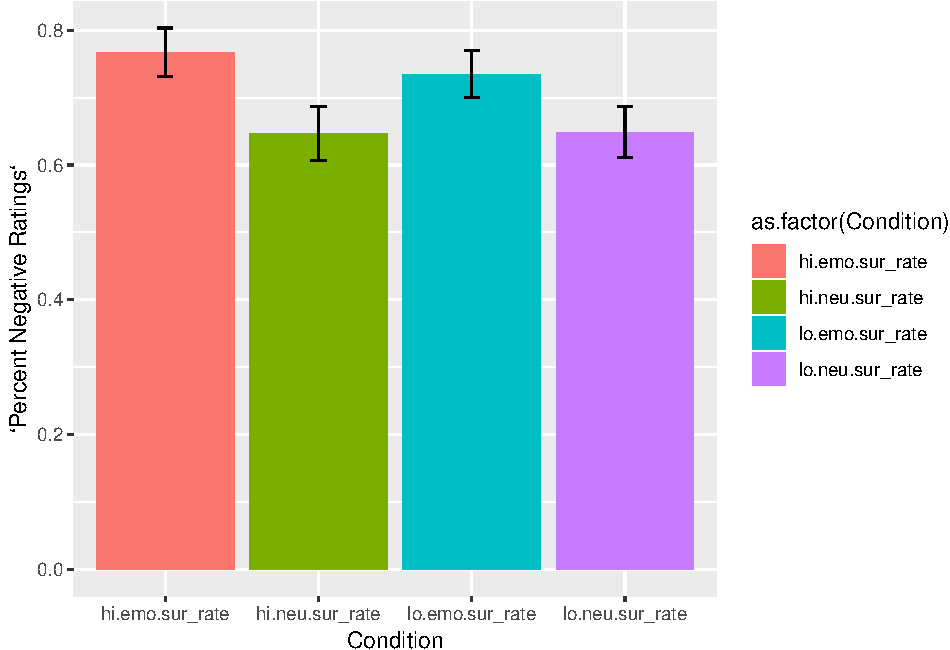
\includegraphics{Manuscript_files/figure-latex/plot figure 1-1.pdf}

\hypertarget{reaction-times}{%
\subsection{Reaction times}\label{reaction-times}}

To assess for normality, the data were first tested with Shapiro-Wilk's test. Two conditions did not appear to be sampled from normal distributions, so non-parametric tests were used. Overall, there was a trending difference across the four conditions, \(\chi^{2}\)(3.00) = 7.15, p .067. Wilcoxon signed rank tests were used to assess post-hoc comparisons and Bonferroni corrected p-value = 0.01. While none of the post-hoc comparisons reached the adjusted significance level, there was a trending difference between emotional and neutral RTs in the high load condition, Z = 2.51, p = .012, such that high emotional WM loads had slower RTs. Two other comparisons were trending for traditional levels of significance. Low emotional WM loads tended to take marginally longer than high neutral WM loads, Z = 1.96, p = .050, and low neutral WM loads took marginally longer than high neutral WM laods, Z = -1.75, p = 0.08. All other comparisons were not significant.

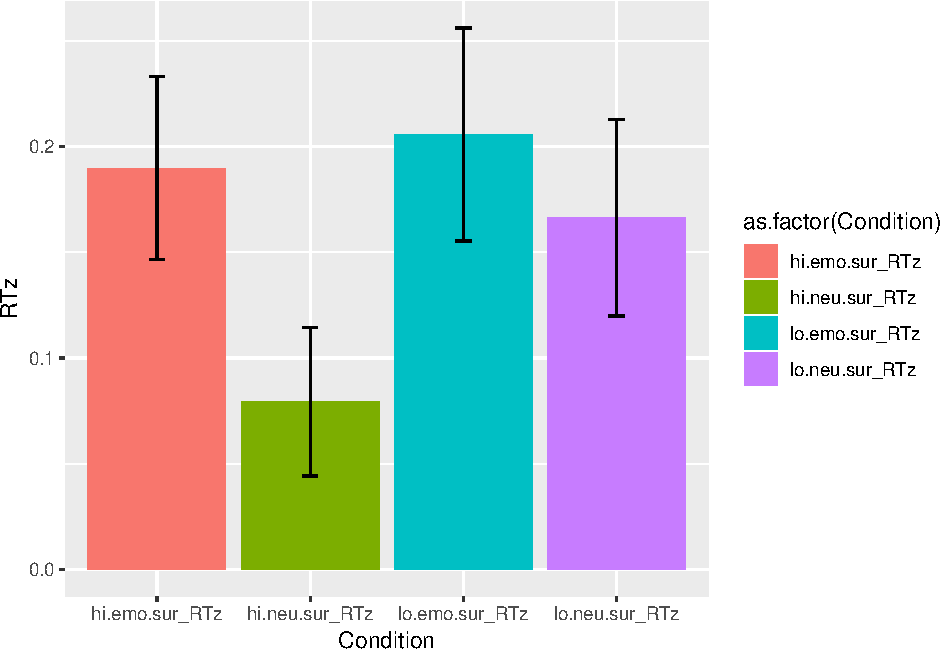
\includegraphics{Manuscript_files/figure-latex/plot RT data-1.pdf}

Next, we tested for reaciton time differences between positive and negative interpretations of surprised facial expressions within each working memory load condition. Given the non-normality of these data, we used paired-sample Wilcoxon signed rank tests for assessing differences between positive and negative ratings of surprise RTs. This difference was significant \emph{only} for the low emotional load trials, with surprise rated as positive taking signficantly longer than surprise rated as negative (.009). All other comparisons were not significant (p's \textgreater{} .200). Further, this effect survived Bonferroni correction (p = .012).

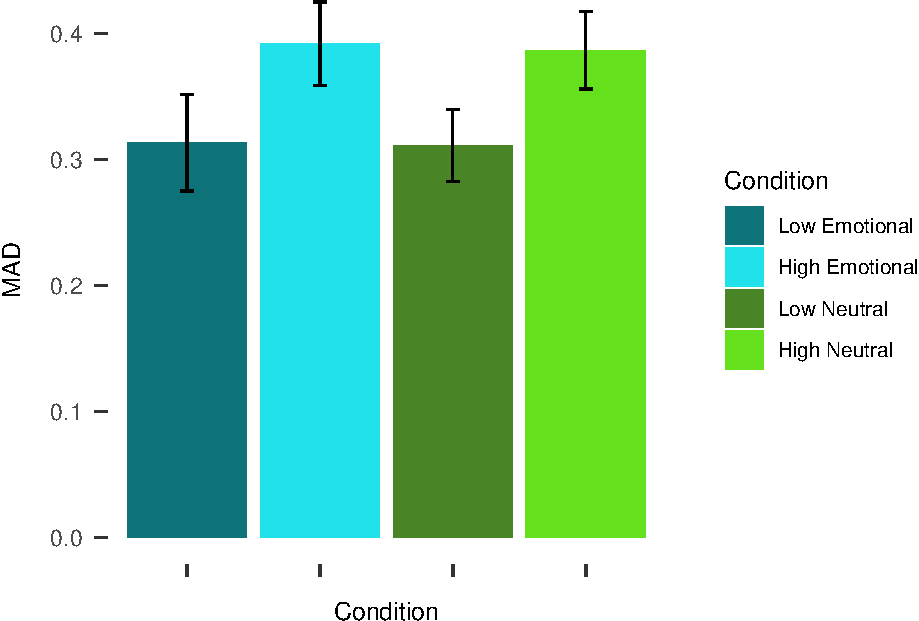
\includegraphics{Manuscript_files/figure-latex/MAD plot-1.pdf}
Finally, we assessed differences in maximum absolute deviation (MAD) across the WM trial conditions.

\hypertarget{discussion}{%
\section{Discussion}\label{discussion}}

The effect of high vs.~low load is still not apparent in these data, just like Mattek et al.~2016. An alternative explanation is that the high load manipulation is not sufficiently difficult to recruit the targeted cognitive resources; however, future work will be needed to better test this alternative.

Previous work has shown that more positive interpretations of surprised faces are related to slower RTs. Our working hypothesis suggests that this delayed reaction is a result of deliberation and slower, top-down cognitive processing. It is interesting to note that, at least in these data, there is no such difference observed between the neutral and emotional WM trials, \emph{even though} the emotional WM trials are overall more negative. Future work should tease apart why this may be. For instance, \ldots{}

\newpage

\hypertarget{references}{%
\section{References}\label{references}}

\begingroup
\setlength{\parindent}{-0.5in}
\setlength{\leftskip}{0.5in}

\hypertarget{refs}{}
\leavevmode\hypertarget{ref-brown_cortisol_2017}{}%
Brown, C. C., Raio, C. M., \& Neta, M. (2017). Cortisol responses enhance negative valence perception for ambiguous facial expressions. \emph{Scientific Reports}, \emph{7}(1), 15107. doi:\href{https://doi.org/10.1038/s41598-017-14846-3}{10.1038/s41598-017-14846-3}

\leavevmode\hypertarget{ref-egner_dissociable_2008}{}%
Egner, T., Etkin, A., Gale, S., \& Hirsch, J. (2008). Dissociable neural systems resolve conflict from emotional versus nonemotional distracters. \emph{Cerebral Cortex (New York, N.Y.: 1991)}, \emph{18}(6), 1475--1484. doi:\href{https://doi.org/10.1093/cercor/bhm179}{10.1093/cercor/bhm179}

\leavevmode\hypertarget{ref-freeman_mousetracker:_2010}{}%
Freeman, J. B., \& Ambady, N. (2010). MouseTracker: Software for studying real-time mental processing using a computer mouse-tracking method. \emph{Behavior Research Methods}, \emph{42}(1), 226--241. doi:\href{https://doi.org/10.3758/BRM.42.1.226}{10.3758/BRM.42.1.226}

\leavevmode\hypertarget{ref-gruber_effects_2001}{}%
Gruber, O. (2001). Effects of domain-specific interference on brain activation associated with verbal working memory task performance. \emph{Cerebral Cortex (New York, N.Y.: 1991)}, \emph{11}(11), 1047--1055. doi:\href{https://doi.org/10.1093/cercor/11.11.1047}{10.1093/cercor/11.11.1047}

\leavevmode\hypertarget{ref-lang_international_2008}{}%
Lang, P., Bradley, M. M., \& Cuthbert, B. N. (2008). International affective picture system (IAPS): Affective ratings of pictures and instruction manual., Technical Report A--8. University of Florida, Gainesville, FL.

\leavevmode\hypertarget{ref-lundqvist_karolinska_1998}{}%
Lundqvist, D., Flykt, A., \& Öhman, A. (1998). The karolinska directed emotional faces---KDEF (CD ROM)., Stockholm: Karolinska Institute, Departmentof Clinical Neuroscience, PsychologySection.

\leavevmode\hypertarget{ref-mattek_differential_2016}{}%
Mattek, A. M., Whalen, P. J., Berkowitz, J. L., \& Freeman, J. B. (2016). Differential effects of cognitive load on subjective versus motor responses to ambiguously valenced facial expressions. \emph{Emotion}, \emph{16}(6), 929--936. doi:\href{https://doi.org/10.1037/emo0000148}{10.1037/emo0000148}

\leavevmode\hypertarget{ref-neta_neural_2013}{}%
Neta, M., Kelley, W. M., \& Whalen, P. J. (2013). Neural responses to ambiguity involve domain-general and domain-specific emotion processing systems. \emph{Journal of Cognitive Neuroscience}, \emph{25}(4), 547--557. doi:\href{https://doi.org/10.1162/jocn_a_00363}{10.1162/jocn\_a\_00363}

\leavevmode\hypertarget{ref-neta_corrugator_2009}{}%
Neta, M., Norris, C. J., \& Whalen, P. J. (2009). Corrugator muscle responses are associated with individual differences in positivity-negativity bias. \emph{Emotion (Washington, D.C.)}, \emph{9}(5), 640--648. doi:\href{https://doi.org/10.1037/a0016819}{10.1037/a0016819}

\leavevmode\hypertarget{ref-neta_dont_2016}{}%
Neta, M., \& Tong, T. T. (2016). Don't like what you see? Give it time: Longer reaction times associated with increased positive affect. \emph{Emotion (Washington, D.C.)}, \emph{16}(5), 730--739. doi:\href{https://doi.org/10.1037/emo0000181}{10.1037/emo0000181}

\leavevmode\hypertarget{ref-stroop_studies_1935}{}%
Stroop, J. R. (1935). Studies of interference in serial verbal reactions. \emph{Journal of Experimental Psychology}, \emph{18}(6), 643--662. doi:\href{https://doi.org/10.1037/h0054651}{10.1037/h0054651}

\leavevmode\hypertarget{ref-tottenham_nimstim_2009}{}%
Tottenham, N., Tanaka, J. W., Leon, A. C., McCarry, T., Nurse, M., Hare, T. A., \ldots{} Nelson, C. (2009). The NimStim set of facial expressions: Judgments from untrained research participants. \emph{Psychiatry Research}, \emph{168}(3), 242--249. doi:\href{https://doi.org/10.1016/j.psychres.2008.05.006}{10.1016/j.psychres.2008.05.006}

\leavevmode\hypertarget{ref-whalen_emotional_2006}{}%
Whalen, P. J., Bush, G., Shin, L. M., \& Rauch, S. L. (2006). The emotional counting stroop: A task for assessing emotional interference during brain imaging. \emph{Nature Protocols}, \emph{1}(1), 293--296. doi:\href{https://doi.org/10.1038/nprot.2006.45}{10.1038/nprot.2006.45}

\endgroup


\end{document}
